\chapter{LANDASAN TEORI}
\section{Computer Vision}
\emph{Computer vision} adalah teknologi yang membuat computer dapat melihat layaknya mata manusia. Penggunaan computer vision tanpa kita sadari telah di implementasikan dalam membantu menyelesaikan persoalan sehari hari. Contoh implementasi \emph{computer vision} antara lain \emph{face recognition, object classification, medical imaging,gesture recognition, video surveillance , 3D reconstruction}. Pada pengolahan citra, sebuah citra memiliki fitur fitur dari penting yang digunakan sebagai informasi saat pengolahan. Namun untuk mendapatkan suatu hasil, beberapa tahap proses harus dilakukan seperti \emph{preprocessing}, ekstraksi ciri, \emph{post-processing} dan sebagainya.
\section{Citra Digital}
Citra dapat didefinisikan sebagai fungsi \(f(x,y)\) berukuran \(M\) baris dan \(N\) kolom, dengan \(x\)  dan \(y\) adalah koordinat spasial dan amplitudo \(f\)  di titik koordinat \((x,y)\) dinamakan tingkat keabuan dari suatu citra. Apabila nilai \((x,y)\) dan \(f\) secara keseluruhan berhingga dan bernilai diskrit maka citra tersebut adalah citra digital. Citra digital dalam bentuk matrik dapat dilihat pada Persamaan 3.1 dan posisi koordinat citra digital dapat dilihat pada gambar 3.1(Sarifudin.,2015).

% TODO: \usepackage{graphicx} required
\begin{figure}[H]
	\centering
	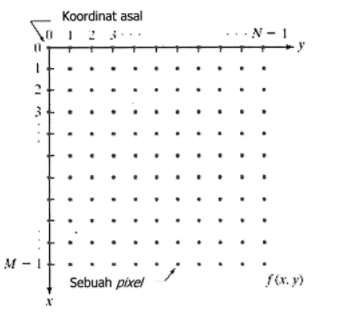
\includegraphics[width=0.3\linewidth]{screenshot001}
	\caption{Koordinat Citra Digital (Sarifudin.,2015)}
	\label{fig:screenshot001}
\end{figure}
\begin{equation}
f(x,y)
\begin{bmatrix}
f(0,0) & f(0,1) & ... & f(0,n-1)\\
f(1,0) & f(1,1) & ... & f(1,n-1)\\
... & ... & ... & ...\\
f(m-1,0) & f(m-1,1) & ... & f(m-1,n-1)\\
\end{bmatrix}
\end{equation}

\subsection{Citra RGB}
Citra RGB disebut juga sebagai citra berwarna, citra ini menyajikan tiga layer warna yaitu Red, Green dan Blue. Setiap piksel dari citra RGB merupakan gabungan dari variasi nilai intensitas tiga warna dasar yaitu merah(R), hijau(G), biru(B). Tiga warna tersebut dikodekan dengan 8 bit,dengan total ketiganya 3 x 8 = 24 bit. Sehingga variasi warna sebanyak $2^{24}$ = 16.777.216 variasi warna (Sarifudin., 2015). Contoh citra RGB dapat dilihat pada Gambar 3.2.
% TODO: \usepackage{graphicx} required
\begin{figure}[H]
	\centering
	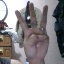
\includegraphics[width=0.35\linewidth]{29}
	\caption{Citra RGB}
	\label{fig:29}
\end{figure}

\subsection{Citra HSV}
Ruang warna HSV memiliki tiga komponen warna, yaitu Hue(H), Saturation(S) dan Value(V).
Hue memiliki variasi warna yang digambarkan secara melingkar, dimana merepresentasikan warna dari merah, kuning, hijau, cyan, biru, magenta,dan kembali lagi ke merah.
Saturation memiliki variasi nilai 0 hingga 1, dimana merepresentasikan saturasi warna dari merah ke merah muda dan Value memiliki nilai 0 hingga 1 yang merepresentasikan intensitas warna atau tingkat kecerahan dari hitam ke putih, dimana nilai semakin tinggi semakin cerah (Kolkur et al., 2017).
Ruang warna HSV dapat di gambarkan seperti Gambar 3.3.
% TODO: \usepackage{graphicx} required
\begin{figure}
	\centering
	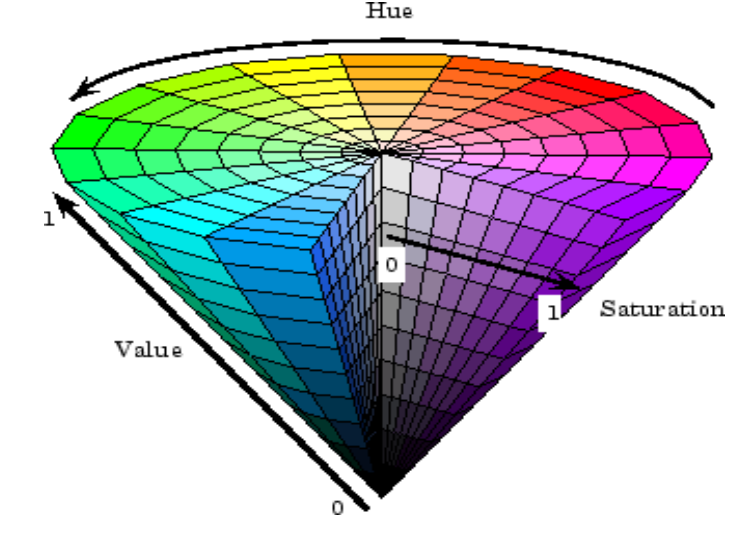
\includegraphics[width=0.45\linewidth]{hsv}
	\caption{Ruang warna HSV (Kolkur et al., 2017)}
	\label{fig:hsv}
\end{figure}

Pada RGB suatu warna di representasikan dengan nilai tiap komponen, namun untuk ruang warna HSV memiliki nilai yang berbeda dari RGB. Hue memiliki range dari 0$^\circ$ sampai 360$^\circ$. Transformasi warna dari RGB ke HSV dapat dilihat dalam Persamaan 3.2, 3.3, 3.4, 3.5.
\begin{equation}
	V = max(R,G,B)
\end{equation}
\begin{equation}
	S=
	\begin{cases}
	\frac{max(R,G,B) - min(R,G,B)}{max(R,G,B)} &  V \ne 0\\
	0 & lainnya
	\end{cases} 	
\end{equation}
\begin{equation}
	H=
	\begin{cases}
	\frac{60(G-B)}{V-min(R,G,B)} &  V=R \\
	120+\frac{60(B-R)}{V-min(R,G,B)} &  V=G \\
	240+\frac{60(R-G)}{V-min(R,G,B)} &  V=B \\
	\end{cases}
\end{equation}
\begin{equation}
	H = H+360
\end{equation}
Penggunaan citra dengan ruang HSV mampu memisahkan informasi warna sesuai dengan kemampuan mata manusia(Afrianto \& Amalia., 2016).
%=====================================operasi morfologi=======================================
\section{Operasi Morfologi}
\subsection{Erosi}
Operasi erosi adalah operasi penipisan objek yang terdapat pada citra biner. Operasi erosi dilakukan dengan cara mengurangi piksel pada kontir dari objek citra sesuai dengan kernel. Operasi erosi dinotasikan pada Persamaan 3.6 (Hidayatullah., 2017).
\begin{equation}
A \ominus B = A^c \oplus B^c
\end{equation}
\subsection{Dilasi}
Operasi dilasi adalah operasi penebalan  objek yang terdapat pada citra biner. Operasi ini dilakukan dengan menambah piksel pada kontur dari objek sesuai dengan kernel. Operasi ini berguna untuk menghaluskan citra dan menutupi lubang-lubang yang kosong. Operasi dilasi dinotasikan pada Persamaan 3.7 (Hidayatullah., 2017).
\begin{equation}
A \oplus B = t \ \epsilon \ Z^2 : t = a + b, a \ \epsilon \ A, \ b \ \epsilon \ B
\end{equation}

\subsection{\emph{Opening}}
Operasi \emph{opening} merupakan operasi yang biasa digunakan untuk memperhalus kontur citra serta menghilangkan lubang-lubang kecil pada citra. Operasi ini terdiri dari 2 dua tahap yaitu erosi kemudian dilanjutkan dilasi. Operasi erosi berguna untuk menghilangkan noise pada citra karena struktur latar depan yang berukuran kecil tereliminasi, sedangkan dilasi digunakan untuk menebalkan citra. Operasi opening dinotasikan dalam Persamaan 3.8(Hidayatullah., 2017).
\begin{equation}
A \bullet B = (A \ominus B) \oplus B
\end{equation}

\subsection{\emph{Closing}}
Operasi \emph{closing} merupakan kebalikan dari operasi \emph{opening}. Terdiri dari dua tahap yaitu operasi dilasi kemudian dilanjutkan dengan operasi erosi. Kegunaan operasi ini adalah untuk menutupi lubang yang kosong pada citra dengan menggunakan dilasi kemudian dilakukan erosi citra untuk menipiskan suatu citra. Operasi closing dinotasikan pada Persamaan 3.9 (Hidayatullah., 2017).
\begin{equation}
A \bullet B = (A \oplus B) \ominus B
\end{equation}
%=====================================end of operasi morfologi=================================
\section{\emph{Hand Gesture Recognition}}

\subsection{\emph{American Sign Language}(ASL)}
Bahasa isyarat merupakan media komunikasi utama bagi kaum difabel khusunya penyandang tunarungu di dunia. Setiap negara mempunyai bahasa isyarat masing masing. Dengan adanya bahasa isyarat, penyandang tunarungu dapat melakukan komunikasi antar sesama penderita maupun berkomunikasi dengan setiap orang. Bahasa isyarat mulai banyak digunakan pada siaran televisi, seperti acara debat ataupun channel berita dengan dibantu penerjemah bahasa isyarat. Dengan begitu memberi mereka hak yang sama untuk mendapatkan informasi. 

Salah satu bahasa isyarat yang digunakan adalah \emph{American Sign Language}(ASL). \emph{American Sign Language} menjadi salah satu alat bantu pembelajaran komunikasi untuk penggunanya. penggunaan bahasa isyarat dilakukan dengan gerakan gestur tangan yang memiliki makna untuk setiap pose. Pada penelitian ini, bahasa isyarat yang digunakan untuk menguji sistem adalah \emph{American Sign Language}. Pada gestur ASL, mempunyai beberapa bentuk gestur tangan huruf dan angka seperti pada Gambar 3.4.
% TODO: \usepackage{graphicx} required
\begin{figure}[H]
	\centering
	\includegraphics[width=0.7\linewidth]{"asl"}
	\caption{American Sign Language (Barczak et al., 2011)}
	\label{fig:asl}
\end{figure}
%!=============================================== Retinex
\section{Retinex(Single Scale Retinex)}
Algoritme \emph{Retinex} merupakan algoritme yang berusaha untuk mempertahankan ketetapan warna dimana warna suatu objek yang dilihat dalam keadaan pencahayaan yang berbeda(Aribowo et al., 2009). Algoritme \emph{Retinex} ini sering juga disebut dengan \emph{Single Scale Retinex} (SSR) karena hanya memiliki satu kanal. Menurut Land sebuah citra terbentuk sebagai perkalian reflektansi dan iluminasi. Berdasarkan teori \emph{Retinex} dapat dituliskan secara matematis seperti Persamaan 3.10 berikut(Parihar \& Singh., 2018)(Petro et al., 2014):
\begin{equation}
	I(x,y) = L(x,y) \boldsymbol{\cdot} R(x,y)
\end{equation}
\begin{equation}
	\log I(x,y) = \log L(x,y) + \log R(x,y)
\end{equation}
\begin{equation}
	\log R(x,y) = \log I(x,y)-\log L(x,y)
\end{equation}
dimana
\begin{equation}
	L(x,y)=F(x,y) * I(x,y)
\end{equation}
\begin{equation}
F(x,y) = \frac{1}{2\pi \sigma^2}e^{-(\frac{x^2 + y^2}{2\sigma^2})}
\end{equation}
\begin{equation}
	\int F(x,y) dxdy = 1
\end{equation}
sehingga
\begin{equation}
\log R = \log I(x,y) - \log [F(x,y) * I(x,y)]
\end{equation}
Keterangan :\\
\(I(x,y) \ :\) representasi dari kumpulansinyal dari citra asli.\\
\(R(x,y) :\) representasi dari komponen reflektansi dari objek.\\
\(L(x,y) :\) representasi komponen pencahayaan yang memenuhi Persamaan 3.12.\\
\(F(x,y) : \) \emph{gaussian function} yang memenuhi Persamaan 3.13.

Bentuk logaritmik pada Persamaan 3.11 digunakan untuk memisahkan antara komponen pencahayaan dan komponen reflektansinya. Pemisahan ini dilakukan untuk mendapatkan informasi dari citra tersebut sehingga hasil \emph{Single Scale Retinex} dapat dilihat pada Persamaan 3.17, dimana $\log R =$ \(R_{SSRi}\) adalah hasil \emph{Single Scale Retinex} pada kanal \(i\) (Parihar \& Singh., 2018)(Petro et al., 2014).
\begin{equation}
\centering
R_{SSRi}(x,y) = \log I_i(x,y) - \log [F(x,y) * I_i(x,y)]
\end{equation}
%!=============================================== MSR==============================
\subsection{Multiscale Retinex(MSR)}
\emph{Multiscale Retinex} merupakan pengembangan dari \emph{Single Scale Retinex} dengan menggabungkan beberapa scale  yang berbeda dengan pembobotan tertentu, dimana bobot tersebut jika dijumlahkan menghasilkan nilai 1. Sehingga nilai  sangat mempengaruhi detail warna dari sebuah citra. Bentuk matematis dari \emph{multiscale Retinex} dapat dilihat pada Persamaa 3.15 dan 3.16 berikut(Petro et al., 2014):
\begin{equation}
R_{MSRi} = \sum_{n=1}^{N} \omega_n R_{SSRi}=\omega_n [\log I(x,y) - \log (F_n(x,y) * I_i(x,y))]
\end{equation}
Keterangan :
\\
\(R_{MSRi} : \) hasil \emph{Multiscale Retinex} pada kanal i
\\
\(\omega_n \ \ \ \ \ \ \ : \) bobot pada skala n\\
Pada SSR dapat menyediakan kompresi rentang dinamis dan penampakan warna, namun keduanya tidak secara bersamaan. Oleh karena itu \emph{Multiscale Retinex} menggabungkan kompresi rentang dinamis dari \emph{Single Scale Retinex} dengan penampakan warna(Aribowo et al., 2009).
%!=============================================== MSRCR
\subsection{Multiscale Retinex Color Restoration(MSRCR)}
MSRCR merupakan pengembangan dari metode MSR yang mampu memperbaiki kualitas citra yang berhubungan dengan pencahayaan yaitu dengan mempertahankan \emph{color constancy}. \emph{Color constancy} berfungsi untuk mempertahankan komposisi warna suatu citra tetap terlihat sama walaupun kondisi pencahayaan yang berbeda-beda (Saputra., 2016). Perhitungan MSRCR dapat dilihat pada Persamaan 3.19, 3.20, 3.21 dan 3.22(Petro et al., 2014).
\begin{equation}
	R'_{MSRCRi}(x,y) = C_i(x,y) \ R_{MSR_i}(x,y)	
\end{equation}
\begin{equation}
	C_i(x,y) = \beta \ {\log[\alpha I'_i(x,y)]}\\
\end{equation}
\begin{equation}
I'(x,y) =\frac{I_i(x,y)}{\sum_{i=0}^{S}I_i(x,y)}
\end{equation}
\begin{equation}
	R_{MSRCRi}(x,y) = G \ [R'_{MSRCRi}(x,y)-b]
\end{equation}
\noindent Keterangan :\\
$i$ = 3 kanal warna RGB\\
$\alpha$ = konstanta kontrol ketidaklinieran\\
$\beta$ = konstanta gain\\
$G$,$b$ = gain dan offset
%!=============================================== MOBILENET
\section{MobileNet}
\emph{MobileNet} merupakan salah satu arsitektur CNN yang dibangun oleh \emph{Google} dan dikhususkan untuk \emph{mobile device} karena proses komputasi yang ringan. Perbedaan arsitektur \emph{MobileNet} dan CNN pada umumnya terdapat pada penggunaan layer konvolusi dengan ketebalan sesuai input dari citra. Arsitektur SSD \emph{MobileNet} menggunakan \emph{Depthwise layer} dan \emph{Pointwise layer}.
\subsection{Depthwise Separable Convolution}
\emph{Depthwise separable convolution} merupakan kunci utama untuk membangun arsitektur \emph{neural network}. Ide utamanya adalah mengganti operator konvolusi secara menyeluruh dengan memisahkan konvolusi menjadi dua lapisan terpisah. Layer pertama adalah \emph{depthwise convolution}, layer ini memiliki \emph{light-weight filter} dengan menggunakan \emph{single convolutional filter} untuk setiap input channel. Layer kedua menggunakan 1x1 convolution yang disebut dengan \emph{pointwise convolution} dimana layer ini membentuk fitur fitur baru melalui perhitungan kombinasi linear dari input channel. 

Pada konvolusi biasa memiliki input citra $D_F$ x $D_F$ x $M $ fitur map pada $F$ dan menghasilkan $ D_G$ x $D_G$ x $N $ fitur map pada $G$, dimana $D_F$ adalah tinggi dan lebar dari fitur map. $M$ merupakan jumlah input channel(input depth). 
$D_G$ merupakan tinggi dan lebar keluaran fitur map dan $N$ adalah keluaran channel dari fitur map\emph{(output depth)}. Kemudian kernel pada konvolusi biasa $D_K$ x $D_K$ x $M$ x $N$, dimana $D_K$ adalah dimensi kernel, $M$ jumlah input channel dan $N$ jumlah keluaran channel. Total cost dari konvolusi biasa memiliki ketergantungan pada $M$ pada Persamaan 3.23.
\begin{equation}
	D_K \bullet D_K \bullet M \bullet N \bullet D_F \bullet D_F
\end{equation}

\emph{Depthwise separable convolution} terbentuk dari layer \emph{depthwise convolution} dan \emph{pointwise convolution}. \emph{Depthwise convolution} sangat efisien daripada konvolusi biasa, namun pada layer \emph{depthwise} tersebut tidak menghasilkan fitur baru, oleh karena itu digunakan tambahan layer \emph{pointwise convolution} untuk menghitung linier kombinasi dari keluaran \emph{depthwise convolution} menggunakan 1x1 \emph{convolutio}n ,sehingga menghasilkan fitur baru. Total cost dari \emph{depthwise convolution} pada Persamaan 3.24.
\begin{equation}
D_K \bullet D_K \bullet M \bullet D_F \bullet D_F
\end{equation}
Kombinasi kedua layer tersebut dinamakan \emph{deptwise separable convolution} yang memiliki total cost Persamaan 3.25 :
\begin{equation}
D_K \bullet D_K \bullet M \bullet N \bullet D_F \bullet D_F + M \bullet N \bullet D_F \bullet D_F
\end{equation}
\emph{MobileNet} menggunakan 3x3 \emph{depthwise separable convolution} yang mana mereduksi komputasi 8 hingga 9 kali lebih cepat dari konvolusi biasa. Perbedaan konvolusi biasa dan \emph{depthwise separable convolution} digambarkan pada Gambar 3.5(Howard et al., 2017).
% TODO: \usepackage{graphicx} required
\begin{figure}[H]
	\centering
	\includegraphics[width=0.5\linewidth]{"new"}
	\caption{Convolutional standard dan depthwise separable (Howard et al., 2017)}
	\label{fig:new}
\end{figure} 
%!=============================================== MOBILENETV2 
\section{MobileNetV2}
Perbedaan \emph{MobileNet} versi kedua merupakan pengembangan dari \emph{MobileNet} versi pertama. Pada \emph{MobileNet} memiliki modifikasi arsitektur linier \emph{bottleneck} dan \emph{shortcut} koneksi antar \emph{bottleneck} seperti Gambar 3.6.
Sehingga arsitektur dalam \emph{MobileNetV2} menjadi \emph{bottleneck depth-separable convolution residuals}. Arsitektur \emph{bottleneck} dituliskan pada Tabel 3.1.
\begin{table}[H]
	\caption{Blok Arsitektur \emph{Bottleneck MobileNetV2} (Sandler et al., 2018)}
	\vspace{0cm}
	\centering
	\begin{tabular}{|p{3cm}|p{4cm}|p{3cm}|}
		\hline
		Input & Operator & Output \\
		\hline
		$h \ x \ w \ x \ k$ & 1$x$1 Conv2D, ReLU6 & $h \ x \ w$ (tk) \\ 
		\hline	
		$h \ x \ w \ x \ tk$ & 3$x$3 dwise s=s, ReLU6 & $\frac{h}{s} \ x \ \frac{w}{s}$ (tk) \\ 
		\hline	
		$\frac{h}{s} \ x \ \frac{w}{s} \ x \ tk$ & linear 1$x$1 Conv2D & $\frac{h}{s} \ x \ \frac{w}{s}$ k' \\ 
		\hline				
	\end{tabular}
\end{table}
Tabel 3.1 menunjukan blok arsitektur \emph{bottleneck} \emph{MobileNetV2} terdiri dari \emph{fully convolution} dengan 32 filter diikuti 19 layer \emph{residual bottleneck}.
Kernel yang digunakan menggunaka ukuran 3x3 (standard untuk modern network) dan menggunakan dropout dan normalisasi selama pelatihan(Sandler et al., 2018). 
\begin{figure}[H]
	\centering
	\includegraphics[width=0.6\linewidth]{"arsitektur"}
	\caption{Struktur Dasar Pada \emph{MobileNetV2} (Google AI Blog., 2018)}
	\label{fig:arsitektur}
\end{figure}
\noindent Pada bagian \emph{bottleneck} terdapat \emph{input} dan \emph{output}, sedangkan layer di bagian dalam mengenkapsulasi kemampuan model untuk merubah input dari piksel ke gambar. Tambahan \emph{shortcut} antar \emph{bottleneck} memungkinkan saat melakukan \emph{training} menjadi lebih cepat dengan peningkatan akurasi yang lebih baik(Google AI Blog,. 2018).
%!=============================================== ConvNeuralNet
\section{Convolutional Neural Network(CNN)}
\emph{Convolutional Neural Network} (CNN) merupakan jaringan syaraf tiruan yang memiliki arsitektur khusus yang dapat bekerja dengan baik dalam penggunaannya pada pemrosesan data berbentuk larik, seperti data runtun waktu dan citra digital. Dalam arsitekturnya CNN menggunakan operasi matematika konvolusi pada layer jaringan. Operasi konvolusi antara a dan b disimbolkan dengan (a x b). \emph{Convolutional neural network} pada penerapannya menggunakan tiga ide dasar yaitu local receptive fields, shared weights, dan pooling(Nielsen., 2015).
%================================================ LOCAL RESPECTIVE FIELD
\subsection{Local Receptive Fields}
Pada jaringan syaraf tiruan dengan \emph{fully-connected}, input dari jaringan 
digambarkan dengan garis vertikal dari kumpulan neuron. Pada CNN, input digambarkan sebagai persegi dengan ukuran o × o sesuai dengan ukuran input yang 
diberikan. Misalkan terdapat input dengan ukuran 28 × 28 neuron, yang 
berkesesuaian dengan 28 × 28 intensitas piksel pada citra seperti terlihat pada 
Gambar 3.7.
% TODO: \usepackage{graphicx} required
\begin{figure}[h]
	\centering
	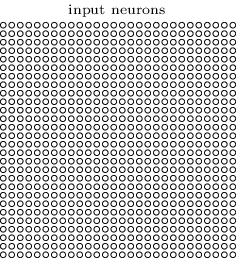
\includegraphics[width=0.25\linewidth]{neuraon}
	\caption{Ilustrasi Citra 28x28 Piksel (Nielsen., 2015)}
	\label{fig:neuraon}
\end{figure}

Seperti jaringan syaraf tiruan pada umumnya, setiap neuron dari input
terhubung dengan layer dari hidden neuron. Sedikit berbeda, pada CNN neuron 
input tidak terhubung secara \emph{fully-connected} dengan setiap hidden neuron, tetapi 
hanya region lokal kecil dari input terhubung dengan sebuah hidden neuron
(Nielsen., 2015). Pada Gambar 3.8 terlihat bahwa hanya sebagian kecil region
yang \emph{localized} dari input neuron yang terhubung dengan hidden neuron.
% TODO: \usepackage{graphicx} required
\begin{figure}[H]
	\centering
	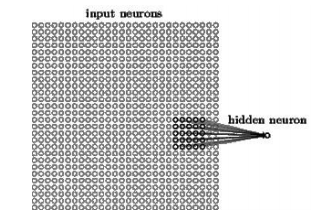
\includegraphics[width=0.5\linewidth]{hidenneuron}
	\caption{Ilustrasi \emph{local receptive fields} (Nielsen., 2015)}
	\label{fig:hidenneuron}
\end{figure}

Pada Gambar 3.9 setiap neuron pada hidden layer terhubung dengan
region berukuran 5 × 5 piksel pada neuron input. Region pada input layer inilah
yang dinamakan dengan \emph{local receptive fields} dan setiap koneksi memiliki bobot
yang akan disesuaikan seiring dengan proses pelatihan. Selain itu hidden neuron 
juga memiliki dan mempelajari bias secara keseluruhan. Oleh karena itu, setiap
hidden neuron dilatih untuk menganalisa masing-masing local receptive fields yang 
bersesuaian.

Tahap selanjutnya, local receptive fields akan digeser (slide) sepanjang 
ukuran citra dari posisi paling kiri atas hingga kanan bawah. Setiap local receptive
fields akan memiliki pasangan hidden neuron yang berbeda pada hidden layer.
Ilustrasi proses pergeseran \emph{local receptive fields} terdapat pada Gambar 3.9 dan
Gambar 3.10 berikut.
% TODO: \usepackage{graphicx} required
\begin{figure}[h]
	\centering
	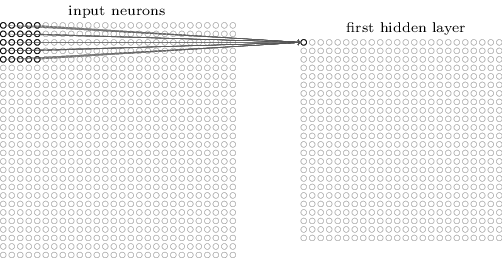
\includegraphics[width=0.65\linewidth]{neuron2}
	\caption{Ilustrasi Pergesaran \emph{local receptive fields} (Nielsen., 2015)}
	\label{fig:neuron2}
\end{figure}

Selanjutnya \emph{local receptive fields} akan digeser sebanyak satu piksel ke
kanan seperti pada Gambar 3.8 dan terhubung dengan hidden neuron yang 
berbeda dengan local receptive fields sebelumnya.
% TODO: \usepackage{graphicx} required
\begin{figure}[h]
	\centering
	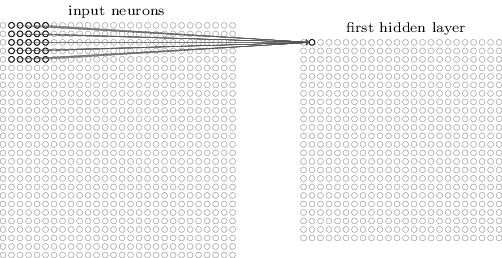
\includegraphics[width=0.65\linewidth]{neuron3}
	\caption{Ilustrasi Pergeseran dengan Stride = 1 (Nielsen., 2015)}
	\label{fig:neuron3}
\end{figure}

Pergeseran piksel dengan stride = 1 di ilustrasikan pada Gambar 3.9.Proses ini berlangsung hingga \emph{local receptive fields} berada pada posisi 
piksel paling kanan bawah. Sehingga setelah proses slide dilakukan akan terbentuk
hidden layer dengan ukuran sesuai dengan ukuran local receptive fields dan 
panjang pergeseran (stride) yang digunakan (Nielsen, 2015). Maka jika citra dengan ukuran 28 × 28 piksel dan digunakan \emph{local receptive fields}
dengan ukuran 5 × 5, dan digeser dengan stride = 1, maka akan terbentuk
hidden layer dengan ukuran 24 × 24 neuron.
%================================================ Shared Weight
\subsection{Shared Weight}
Pada CNN, sebuah neuron pada hidden layer yang terhubung dengan 5 × 5 
neuron pada input layer (sesuai dengan ukuran \emph{local receptive fields} yang 
digunakan). Hal ini menunjukkan bahwa neuron tersebut memiliki sebuah bias dan 
matriks bobot dengan ukuran 5 × 5 yang menghubungkan 5 × 5 neuron inputnya.
Matriks bobot ini, dalam CNN, disebut sebagai kernel. Matriks bobot pada jaringan 
syaraf tiruan biasa sedikit berbeda dengan matriks bobot pada CNN, yaitu nilai 
matriks bobot pada CNN bernilai sama untuk setiap 24 × 24 neuron pada hidden 
layer. Hal tersebut menunjukkan bahwa semua neuron pada hidden layer akan 
mendeteksi fitur yang sama dengan lokasi pada input citra yang berbeda (Nielsen., 
2015).

%!=============================================== Konvolusi
\subsection{Konvolusi}
Lapisan yang pertama kali akan dilewati oleh data masukan adalah lapisan konvolusi, bertujuan untuk memperoleh feature map yang merepresentasikan masukan. Parameter yang digunakan untuk menentukan ukuran feature map keluaran berupa filter, ukuran dari filter, besarnya langkah pergeseran filter pada operasi konvolusi atau biasa disebut stride, dan ukuran padding. Cara menghitung ukuran dari keluaran operasi konvolusi ditunjukkan pada Persamaan 3.26 dan 3.27  berikut(Nielsen., 2015):
\begin{equation}
H_0 = \frac{H-F+2P}{S}+1
\end{equation}

\begin{equation}
W_0 = \frac{W_i-F+2P}{S}+1
\end{equation}
Keterangan : \\
\(H_0\) = tinggi fitur map keluaran
\\
\(W_0\) = lebar fitur map keluaran\\
\(H_i\) = tinggi fitur map masukan
\\
\(W_i\) = lebar fitur map masukan
\\
\(F\)  = ukuran filter
\\
\(P\)  = ukuran padding
\\
\(S\)  = ukuran stride 

Nilai semua elemen pada persamaan tersebut harus merupakan bilangan bulat karena akan merepresentasikan suatu ukuran feature map. Apabila terdapat salah satu nilai yang bukan merupakan bilangan bulat, nilai tersebut harus dibulatkan dengan melakukan pembulatan kebawah. Adapun cara menghitung nilai keluaran dari proses konvolusi dapat dilihat pada Persamaan 3.278berikut(Nielsen., 2015):
\begin{equation}
O_{mn}=\sum I^k_{i,j} . F_{i,j}
\end{equation}
Keterangan :
\\
\(O_{mn}\)= elemen matriks keluaran pada baris ke-m kolom ke –n.
\\
\(I^k_{i,j}\)= elemen matriks masukan bagian ke-k pada baris ke-i kolom ke-j. 
\\
\(F_{i,j}\)= elemen matriks filter pada baris ke-i kolom ke –j.
%!=============================================== Fungsi Aktivasi
\subsection{Fungsi Aktivasi}
Salah satu faktor signifikan mempengaruhi kinerja algoritme Convolutional Neural Network adalah penerapan fungsi aktivasi dalam jaringan. Fungsi ini membantu menyelesaikan permasalah-permasalahan yang bersifat non-trivial dalam suatu jaringan dengan cara mengambil sebuah nilai dan melakukan operasi matematika. Fungsi aktivasi ini diletakkan di perhitungan akhir dari keluaran feature map atau setelah layer konvolusi dan subsampling layer. Fungsi aktivasi yang sering digunakan adalah Rectified Linear Unit (ReLU) karena fungsi ini lebih cepat daripada fungsi aktivasi non-linear lainnya seperti sigmoid atau tanh. Fungsi ReLU dapat dilihat pada Persamaan 3.29 dan 3.30(Nielsen., 2015):
\begin{equation}
f(x) = ReLU(x) =max(0,x)
\end{equation}
\begin{equation}
	f(x)= 0 \ jika \ x \leq{0} \ atau \ x \ jika > 0
\end{equation}
\section{Evaluasi}
\subsection{Confussion Matrix}
Pengukuran evaluasi dari pengujian dapat dilakukan menggunakan \emph{confusion matrix}. tabel \emph{confusion matrix} merupakan tabel klasifikasi yang bersifat prediktif seperti ditunjukan pada Gambar 3.11. Evaluasi menggunakan confussion matrix dapat digunakan untuk mengukur nilai akurasi dengan Persaman 3.31.
% TODO: \usepackage{graphicx} required
\begin{figure}[H]
\centering
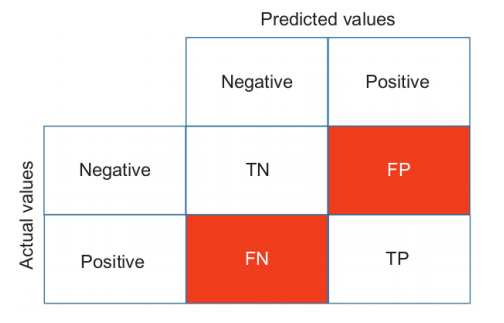
\includegraphics[width=0.7\linewidth]{confusion}
\caption{Confusion Matrix (Leonard., 2017)}
\label{fig:confusion}
\end{figure}
\begin{equation}
akurasi = \frac{TP}{TP+FP}
\end{equation}
Dengan :\\
$TP$ = True Positif, objek berupa gestur tangan dan terkenali\\
$FP$ = False Positif, objek berupa gestur tangan tapi tidak terkenali
\subsection{Average Precicion(AP)}
\emph{Average Precicion} adalah metrik populer untuk melakukan evaluasi pada objek detektor seperti \emph{Faster-RCNN, SSD, dan lainnya}. AP menghitung nilai rata rata nilai presisi untuk nilai recall 0 hingga 1 (Hui., 2018). Evaluasi deteksi menggunakan konsep IoU(\emph{intersection over union})
IoU menghitung interseksi kedua bounding boxes dimana terdiri dari ground truth dan prediksi dari bounding box digambarkan pada Gambar 3.12 dan perhitungan IoU pada Persamaan 3.32.
% TODO: \usepackage{graphicx} required
\begin{figure}[H]
	\centering
	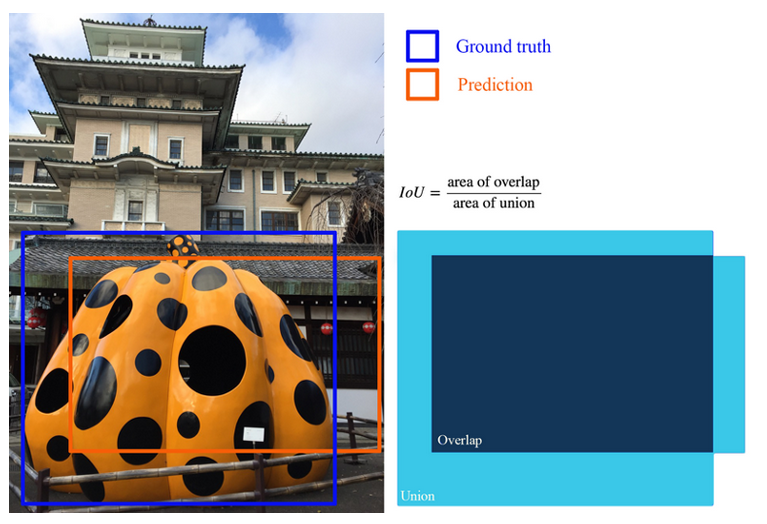
\includegraphics[width=0.7\linewidth]{iou}
	\caption{Ilustrasi IoU(Hui., 2018)}
	\label{fig:iou}
\end{figure}
\begin{equation}
	IoU=\frac{area\_of\_overlap}{area\_of\_union}
\end{equation}

IoU yang digunakan untuk memprediksi suatu bounding box, apabila nilai IoU melebihi \emph{threshold} yang ditentukan maka akan terdeteksi sebuah objek.
Sebaliknya jika IoU kurang dari batas yang ditentukan maka menandakan tidak terdeteksi apapun pada citra. 

Terdapat 4 kategori dalam penentuan deteksi yaitu,
FN(\emph{False Negative}) terdapat objek namun tidak mendeteksi apapun.
FP(\emph{False Positive}) tidak terdapat objek namun hasilnya terdeteksi.
TP(\emph{True Positive}) terdapat objek dan terdeteksi.
TN(\emph{True Negative}) akan terjadi jika tidak ada objek dan tidak terdeteksi apapun.
Berdasarkan nilai yang didapat maka diketahui presisi dan recall menggunakan Persamaan 3.33 dan Persamaan 3.34 (Hui., 2018).
\begin{equation}
	presisi = \frac{TP}{TP+FP}
\end{equation}
\begin{equation}
recall = \frac{TP}{TP+FN}
\end{equation}
Metrik untuk mengukur detektor dari \emph{object detection} menggunakan mAP \emph{(mean average precicion)}. Nilai mAP dan AP dalam COCO dataset tidak memiliki perbedaan, dimana mAP adalah rata rata dari setiap AP yang memiliki nilai IoU sebagai \emph{threshold}. Total metrik evaluasi pada COCO memiliki 12 metrik seperti pada Gambar 3.13 (Chen et al., 2015).
% TODO: \usepackage{graphicx} required
\begin{figure}[H]
	\centering
	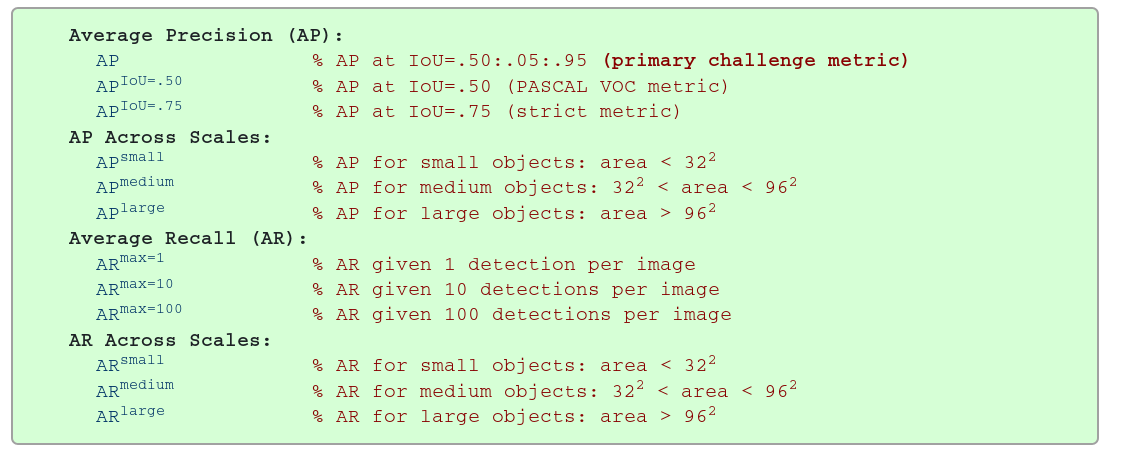
\includegraphics[width=1\linewidth]{mtrik}
	\caption{Metrik Evaluasi COCO (Chen et al., 2015)}
	\label{fig:mtrik}
\end{figure}

